% Compile from this directory with: xelatex why_three_stage3.tex
\documentclass[11pt,a4paper]{article}
\usepackage{kotex}
\usepackage{amsmath,amssymb,booktabs,graphicx,geometry,hyperref}
\geometry{margin=25mm}
\graphicspath{{../results/}}
\hypersetup{colorlinks=true,urlcolor=blue}

\title{I01 후속 실험 3: 주기적 토러스의 반대 감김 끈은 언제 소멸 가능한가?}
\author{접촉 기하와 조건부 감김 제거 단계의 분리}
\date{2026년 10월 2일}

\begin{document}
\maketitle

\begin{abstract}
앞의 국소 접선 실험을 단위 공간 토러스 $T^d$의 반대 감김
$(+1,-1)$ 끈 쌍으로 확장했다. 주기영상, 유한 관측시간,
두 조화의 주기적 횡방향 굴곡을 포함하고, 끈 조각을 선형화한
각 구간의 최소거리를 정확히 최적화한다. 접촉률은 $d=3$에서
$d=4,5$보다 높지만, 이것만으로 감김이 소멸하거나 반지름이
팽창하지 않는다. 접촉 후 소멸 효율과 가능한 접촉 기회 수를
별도로 놓으면 3에서 멈추는 조건 창이 생기며, 그 창은 효율이
낮을 때 쉽게 닫힌다.
\end{abstract}

\section{문헌 위치와 실험 경계}
감김 소멸률의 차원이 $d>3$에서 억제된다는 분석과
dilaton--gravity에 결합한 끈 기체 연구가 이미 있다
\cite{Greene2010}. 동시에 작은 공간에서 끈의 양자역학과
실제 상호작용률 때문에 통상적인 열평형 가정이 성립하지
않을 수 있다는 분석도 있다 \cite{Danos2004}.
따라서 아래 코드는 기존 메커니즘을 \emph{단순화해서 검증하는
기준선}이다. 원래 I01의 대각 게이지 제약을 설명하는 모형도,
초기 우주의 충실한 끈 이론 계산도 아니다.

\section{구체적인 $T^d$ 끈 쌍}
단위 토러스의 한 방향에 감김수 $+1,-1$을 가진 두 끈을 둔다.
종방향 위치를 맞추는 매개변수 재지정 후, 동일 시간에서
두 끈 사이의 횡방향 변위는
\begin{equation}
\Delta x_\perp(t,s)=c+vt+h(s)\pmod{\mathbb Z^{d-1}},
\qquad (t,s)\in[0,1]^2
\end{equation}
로 쓴다. $c_j\sim U[-1/2,1/2]$, $v_j\sim U[-1/4,1/4]$이며,
$h(s)$는 두 개의 Fourier 조화로 만든 주기함수다.
절대 진폭을 $\epsilon=0,0.05,0.15$로 정규화한다.
이 $h$는 두 끈의 횡방향 형상 차이만 모델링한다.
종방향 속도, Nambu--Goto 운동, 재연결 진폭, 중력 반작용은 없다.

두 끈이 관측기간 안에 접촉했다는 사건은
\begin{equation}
\min_{t,s\in[0,1]}\min_{\ell\in\mathbb Z^{d-1}}
\|c+vt+h(s)-\ell\|\le\delta
\end{equation}
이다. $h$를 기본 12구간의 주기적 선분으로 보간한다.
각 구간과 주기영상에 대해 시간--선분 좌표의 2변수 box
최소제곱을 내부/네 변에서 정확히 구한다.
생성된 경로의 각 좌표 절댓값은 1보다 작으므로 필요한
최근접 주기영상은 축당 $-1,0,1$이다.
접촉은 \emph{감김 소멸 가능성}의 기하적 사건일 뿐이다.
실제 소멸을 가정할 때는 $+1$과 $-1$을 함께 제거해
총 감김수 0을 보존한다.

\section{접촉률과 수치 오차}
고정 seed 20261004, $d=3$ 20,000쌍, $d=4$ 50,000쌍,
$d=5$ 20,000쌍으로 $\delta=0.02$를 측정했다.
괄호는 이 독립쌍 표본의 Wilson 95\% 구간이다.
\begin{center}
\begin{tabular}{@{}cccc@{}}
\toprule
굴곡 $\epsilon$ & $d=3$ & $d=4$ & $d=5$\\
\midrule
0 & $0.0100\;(0.00871,0.01148)$ &
$0.00026\;(0.000152,0.000445)$ & $0.00005$\\
0.05 & $0.02965$ & $0.00200$ & $0.00010$\\
0.15 & $0.0818\;(0.0781,0.0857)$ &
$0.0067\;(0.00602,0.00745)$ &
$0.00035\;(0.000170,0.000722)$\\
\bottomrule
\end{tabular}
\end{center}
$d=5$의 매우 작은 확률은 사건 수가 적으므로
정밀한 값보다 상한/규모로 읽어야 한다.
선형 구간의 최소거리가 $10^{-7}$ 이하인 영두께 교차를
별도로 세면 $d=3$에서 $\epsilon=0,0.05,0.15$ 순서로
$0,0.01765,0.05775$였다. 같은 표본의 $d=4,5$에서는
모두 0이었다. 이 결과는 굽은 감김쌍의 $d=3$ 교차가
유한두께 검출기의 인공물만은 아니라는 기하학적 확인이다.
다만 유한 선분 근사에서의 교차이며 재연결을 뜻하지 않는다.
상대 운동도 필요하다. $\epsilon=0.15$를 고정하고 횡방향
상대속도의 성분 범위를 $[-v_{\max},v_{\max}]$로 바꾼
별도 5,000쌍 실험에서, $v_{\max}=0,0.1,0.25,0.5$의
$d=3$ 영두께 교차율은 각각
$0,0.0296,0.0586,0.0938$이었다.
$v_{\max}=0$에서는 굴곡이 있어도 시간 매개변수가
독립 방향을 제공하지 않으므로 영두께 교차가 사라진다.
같은 순서의 $\delta=0.02$ 접촉률은
$0.0318,0.0510,0.0844,0.1256$이다.
굴곡은 $d=3$의 절대 접촉률을 키우지만 $d=4$도 함께 키운다.
그래서 $p_3/p_4$의 비율만으로 선택성을 판단하면 안 된다.
\emph{유한 시간 안에} $d=3$의 감김이 충분히 사라지는지도 필요하다.

같은 5,000쌍에 대해 $\epsilon=0.15$에서 선분 수를 6,12,24로
바꾸면 $\delta=0.02$의 $d=3$ 접촉률은
$0.0722,0.0812,0.0830$, $d=4$는
$0.0050,0.0056,0.0060$이었다. 선분 12는 정성적 결론에는
충분하지만 정확한 접촉률에는 잔여 보간 오차가 있다.
표본오차 구간 역시 보간 오차를 포함하지 않는다.

\section{접촉에서 팽창까지: 추가로 가정한 단계 규칙}
한 축마다 $K$개의 독립적인 반대 감김쌍이 있고 각 쌍이 평균
$M$개의 독립 접촉 기회를 Poisson 분포에 따라 갖는다고
\emph{가정}한다. 한 접촉이 실제 소멸로 이어질 확률을
$\eta_{\rm ann}$이라 하면 한 쌍의 제거 확률과 $d$방향
전체 감김 제거 확률은
\begin{equation}
q_d=1-e^{-M\eta_{\rm ann}p_d},\qquad
S_d=q_d^{dK}.
\end{equation}
``제거되면 해당 $d$차원 팽창이 안정화된다''는 가정을
\emph{또} 넣으면, 이미 3단계에 도달했다는 조건 아래
\begin{equation}
P_{\rm stop\,3}=S_3(1-S_4)
\end{equation}
를 쓸 수 있다. 이는 실제 우주가 3차원이 될 확률이 아니다.

$\delta=0.02$, $M=30$, $K=1$, $\eta_{\rm ann}=1$에서는
$\epsilon=0,0.05,0.15$ 순서로 이 조건부 값이
$0.0174,0.2045,0.7628$이다. $\epsilon=0.15$라도
$\eta_{\rm ann}=0.1$이면 $0.0103$으로 줄고,
$K=2$이면 $0.5832$가 된다.
반대로 $M$을 모형에 맞춰 자유롭게 최적화하면
곧은 끈도 $M\simeq857$에서 거의 1에 이른다.
그렇지만 $M=30$에서는 거의 실패한다.
이 비교는 최대 확률보다 이용 가능한 상호작용 횟수와
소멸 효율을 먼저 계산해야 함을 보여준다.

\begin{figure}[ht]
\centering
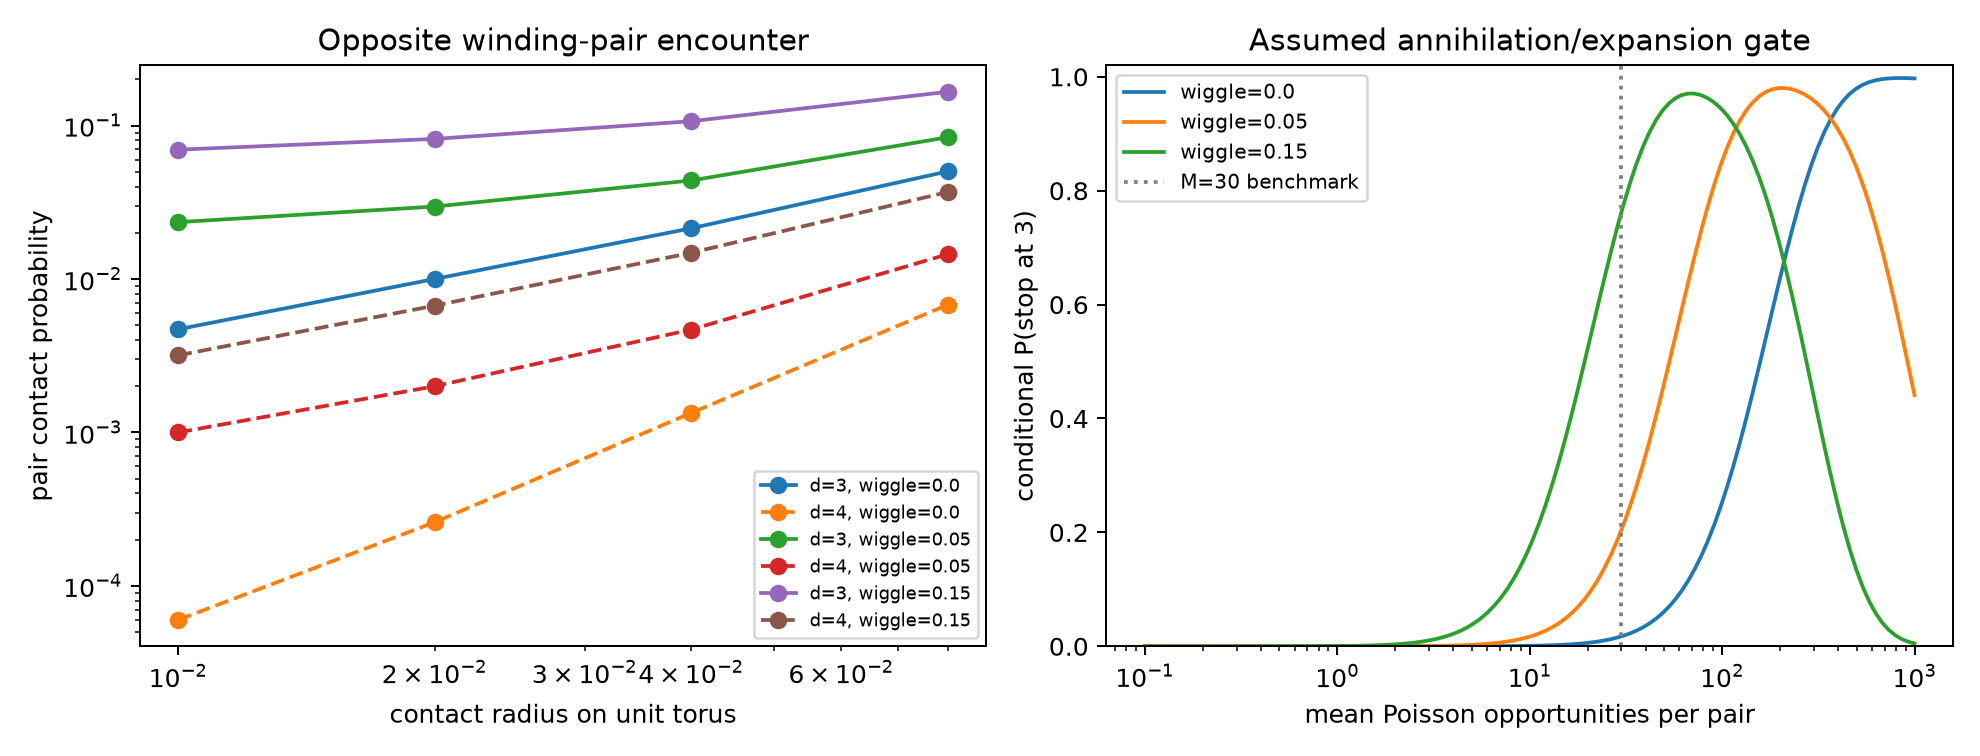
\includegraphics[width=\textwidth]{torus_winding.png}
\caption{왼쪽: 주기적 토러스에서 반대 감김쌍의 접촉률.
오른쪽: 별도 감김소멸/팽창 규칙 아래의 조건부 단계 결과.
점선은 비교용 평균 접촉 기회 $M=30$이다.}
\end{figure}

\section{현재 판정과 다음 작업}
여기서 확인한 것은 (i) $T^d$의 실제 주기영상을 고려해도
$d=3$과 $d=4$의 접촉률이 분리될 수 있고,
(ii) 곧은/굽은 끈, 접촉 두께, 허용 시간,
실제 소멸 효율과 초기 감김쌍 수가 모두 선택성을 좌우한다는 것이다.
그러나 반지름 $R_i(t)$의 운동방정식, 팽창에 따른 밀도 희석,
감김 에너지, 재연결 단면적, 끈의 실제 진동 모드는 없다.
이 항목들을 넣은 뒤 동일한 초기조건 ensemble에서
\emph{최종 큰 반지름의 개수}를 재야 한다. 또한 I01이 주장하는
관측가능 차원과 물질 전파의 차원을 같은 실현에서 측정해
세 개가 일치하는지 검증해야 한다. 일치하지 않으면
접촉 기하를 공간 발생으로 해석하지 않는다.

\paragraph{재현성.} 코드는 \texttt{../src/relational\_atlas\_i01/geometry/torus\_winding.py},
원자료는 \texttt{../results/torus\_winding.json},
기하/규칙 검사는 \texttt{../tests/test\_torus\_winding.py}에 있다.

\begin{thebibliography}{9}
\bibitem{Greene2010} B. Greene, D. Kabat, and S. Marnerides,
``Dynamical Decompactification and Three Large Dimensions,''
\emph{Phys. Rev. D} \textbf{82}, 043528 (2010),
\url{https://arxiv.org/abs/0908.0955}.
\bibitem{Danos2004} R. Danos, A. R. Frey, and A. Mazumdar,
``Interaction Rates in String Gas Cosmology,''
\emph{Phys. Rev. D} \textbf{70}, 106010 (2004),
\url{https://arxiv.org/abs/hep-th/0409162}.
\end{thebibliography}
\end{document}
